\documentclass[11pt,letterpaper]{article}
\usepackage[utf8]{inputenc}
\usepackage{amsmath}
\usepackage{amsfonts}
\usepackage{amssymb}
\usepackage [english] {babel}
\usepackage{graphicx}
\usepackage{tabularx}
\usepackage{booktabs}
\usepackage{apacite}
\usepackage{xspace}
\usepackage{sectsty}
\usepackage{setspace}
\usepackage{textcomp}
\usepackage{hyperref}
 
\sectionfont{\large}

\begin{document}

\begin{center}
{{\huge \textbf{Medición de la Rotación Diferencial del Sol} \\ 
\singlespacing 
{\large \textbf{María Camila Remolina Gutiérrez\\ 
\normalsize 
\texttt{mc.remolina197@uniandes.edu.co}\\
 }}}}
\end{center}

\hrule

\begin{abstract}
El siguiente artículo tiene como objetivo presentar el proyecto: \textit{Medición de la Rotación Diferencial del Sol}. Se busca introducir al tema, y explicar el método a seguir para obtener el resultado deseado. Todo esto, siendo parte del proyecto final del Seminario de Astronomía y Astrofísica de la Universidad de los Andes.
\\
\end{abstract}

\hrule

\section{Introducción}
El Sol, al igual que diferentes cuerpos celestes como planetas o asteroides, tiene polo norte, polo sur y gira alrededor de un eje. Sin embargo, la velocidad de esta rotación no es constante en toda la superficie debido a que el Sol no es un sólido en totalidad sino que su fotosfera se encuentra en estado plasmático, lo cual ocasiona que el ecuador gire a velocidades mayores que en los polos. 
\\

Esta rotación diferencial tiene como consecuencia que el campo magnético del Sol se enrede alrededor de él mismo, causando dos fenómenos: erupciones solares y manchas solares. Las primeras suceden cuando este campo enredado se revienta y no vuelve a entrar al sol, liberando cantidades enormes de energía. Por otro lado, las manchas solares se producen cuando el campo que se rompió vuelve a entrar a la superficie, produciendo una diferencia de temperatura e intensidad luminosa, que en comparación a la luz total emitida por el sol se ve relativamente oscura.
\\

\hrule

\section{Objetivos}
El objetivo principal del proyecto es poder calcular los diferentes periodos en los que gira la superficie del sol por medio manchas solares con datos experimentales tomados desde el observatorio de la Universidad de los Andes.\\

\hrule

\section{Metodología}

La manera como se llevara a cabo este proyecto se divide en dos etapas: toma de datos y la cálculo de resultados.\\

\subsection{Toma de Datos}

Debido a que este proyecto es en gran parte observacional, la toma de datos es una parte fundamental en el proceso. Para esto, de lunes a viernes 2 veces al día (mañana y tarde) se realizan tomas fotográficas al Sol desde el observatorio astronómico de la Universidad de los Andes. Sin embargo, debido a las condiciones climáticas de la ciudad de Bogotá, en repetidas ocasiones no es posible observar al sol en su totalidad; por esta razón, y también para comparar y poder localizar la imagen tomada en la posición correcta, se utilizan las fotografías satelitales que ofrece el Lockheed-Martin Solar and Astrophysics Laboratory (LMSAL) provistas por el Solar Dynamics Obsbervatory (SDO).
\\

\subsection{Cálculo de Resultados}

Para el análisis de los datos obtenidos, hay que primero introducir el tema de coordenadas heliográficas, que en otras palabras es dividir el mapa del sol en una rejilla que se asemeja a las latitudes y longitudes de la Tierra (Fig. 1).
\\

\begin{figure}[h]
 \centering
 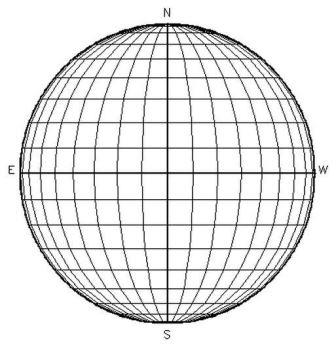
\includegraphics[width=0.7\linewidth]{./grid}
 \caption{Rejilla Solar.}
 \label{fig:grid}
 \end{figure}
 
La idea es escoger un punto dentro de la mancha que esté lo más cerca al centro para tener una representación puntual de ella. A continuación, se mide la posición de cada una de las manchas sobre la rejilla solar a medida que pasa el tiempo, para de esta manera determinar la velocidad angular de cada mancha y con ésta el periodo para cada latitud de acuerdo a las ecuaciones en (1). 
\\

\begin{equation}
\omega =  \frac{\Delta LONGITUD}{\Delta TIEMPO} 
\quad
\quad
T =  \frac{360}{\omega} 
\end{equation}

\subsubsection{Software Utilizado}
 
Para la medición de cada latitud y longitud de las manchas se utilizó el freeware HelioViewer provisto por Peter Meadows.
\\

\subsubsection{Incertidumbres de mediciones}
 
A continuación están las incertidumbres para la medición de cada latitud y longitud del HelioViewer y la del tiempo provista por el SDO:
\\

\begin{equation}
\Delta LONGITUD =  \pm 1^{\circ}\mathrm{}
\quad
\quad
\Delta TIEMPO =  \pm 1 \times 10^{-4} seg
\end{equation}

 
\hrule

\section{Resultados}

A partir de las observaciones se escogen la mayor cantidad de manchas que sean constantes durante el tiempo de observación y se tabula su respectiva latitud (Tab. 1). Por medio de las ecuaciones en (1) se obtienen los valores de velocidad angular y periodo para cada mancha seleccionada y se añaden a la tabla.
\\ 

% Table generated by Excel2LaTeX
\begin{table}[htbp]
  \centering
	\begin{tabular}{cccc}
	\toprule
	    Mancha &  Latitud (°) & w (°/día) &   T (días) \\
	\midrule
	         1 &         15 & 13,3333333 &         27 \\
	         2 &        -16 &         13 & 27,6923077 \\
	         3 &        -15 & 13,3333333 &         27 \\
	         4 &        -16 & 13,0285714 & 27,6315789 \\
	         5 &         16 & 13,1428571 & 27,3913043 \\
	         6 &          8 & 14,6086957 & 24,6428571 \\
	         7 &         12 &         14 & 25,7142857 \\
	         8 &         18 &         12 &         30 \\
	         9 &         -8 & 14,7272727 & 24,4444444 \\
	        10 &         14 &      13,44 & 26,7857143 \\
	        11 &         23 &       10,8 & 33,3333333 \\
	        12 &         10 &         14 & 25,7142857 \\
	        13 &        -17 &         12 &         30 \\
	        14 &        -17 &         12 &         30 \\
	        15 &         26 &         10 &         36 \\
	\bottomrule
	\end{tabular} 
	\caption{Latitud, velocidad angular y periodo para cada mancha.}%

\end{table}%

\subsection{Regresión}

A partir de los datos obtenidos de Latitud vs Velocidad Angular, se realiza una regresión de cuarto grado que para el rango de latitudes escogidos se acomoda de la mejor manera a las velocidades obtenidas (Fig. 2).
\\

\begin{figure}[h]
 \centering
 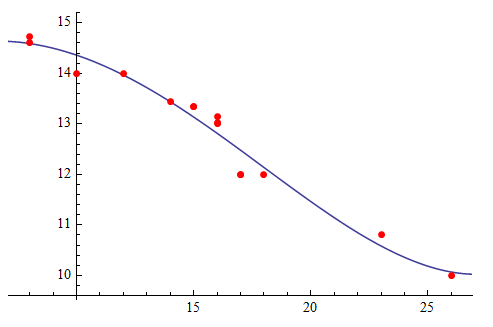
\includegraphics[width=0.522\linewidth]{./latw}
 \caption{Latitud - Velocidad Angular}
 \label{fig:latw}
 \end{figure}
 
Donde el eje x son las latitudes L y el eje y las velocidades angulares w.
\\
 
Se obtiene la ecuación (3) donde se representa la latitud con la letra L. A pesar de estar de acuerdo a los datos obtenidos, solo funciona para un rango de latitudes cercanas a las obtenidas; al extenderse a valores muy grandes de latitud se obtiene un dato incoherente con el teórico. 

\begin{equation}
\omega =  13.4951 + 0.351001 L - 0.0265405 L^2 - 0.000174774 L^3 + 0.0000185153 L^4
\end{equation}

\begin{equation*}
R^2 =  0.961589
\end{equation*}

A partir de está ecuación se tiene un valor de latitud en el ecuador de:

\begin{equation}
\omega_{ec} =  13.4951^{\circ}\mathrm{}/dia \pm 0.052632
\end{equation}
 
En comparación al valor teórico (6) obtenido del modelo más aceptado para rotación diferencial solar (5) se obtiene el error porcentual (7).

\begin{equation}
\omega =  A + B \sin{L}^2 + C \sin{L}^4
\end{equation}

\begin{equation*}
A= 14.713^{\circ}\mathrm{}/dia \pm 0.0491
\quad
\quad
B= –2.396^{\circ}\mathrm{}/dia \pm 0.188
\end{equation*}

\begin{equation*}
C= –1.787^{\circ}\mathrm{}/dia \pm 0.253
\end{equation*}

\begin{equation}
\omega_{teo} =  14.713^{\circ}\mathrm{}/dia \pm 0.0491
\end{equation}

\begin{equation}
error_{\%} =  8.2777 \%
\end{equation}

\hrule

\section{Discusión}

En este proyecto hay varias fuentes de error que pueden afectar el resultado y que se mencionarán a continuación.
\\

\subsection{Observaciones}
En las observaciones realizadas se tiene que tener muy en cuenta que el instrumento utilizado (cámara fotográfica) no tiene la mejor calidad de imagen posible, en particular resolución, lo cual dificulta la medicion de latitud y longitud. Añadido a esto, la forma de colocar el filtro utilizado para visualizar el sol puede en pequeña medida deformar la imagen.
\\

\subsection{Método}
Respecto al método escogido, se puede ver que aunque éste es útil y práctico, no es muy preciso y da cabida a muchos errores. Por esta razón, para hallar las velocidades angulares del Sol se utilizan espectros de manchas en cada latitud.
\\

\subsection{Medición}
En lo que respecta a la medición de latitud y longitud de cada mancha se presentan dos fuentes de error principales. En primer lugar, la precisión con que se pueden determinar las coordenadas heliográficas, como se puede ver en la sección 3.2.2, es 1 grado de incertidumbre, lo cual es muy grande en comparación y puede alterar mucho los resultados. En segundo lugar, el tamaño de la mancha influye a la hora de hallar su centroide (respecto al cual se mediran coordenadas), es decir que para manchas muy grandes la velocidad es muy variable de acuerdo al punto escogido para medir dentro de ella.
\\

\subsection{Regresión - Modelo}
Se puede observar que la regresión obtenida no es coherente para rangos lejanos de las latitudes presentadas en los datos observacionales tomados, ya que para latitudes mucho mayores, el resultado de la velocidad es muy grande. Sin embargo, se puede notar que siguen el mismo comportamiento por un tiempo (grado 4) ; pero para observaciones en cada latitud independiende es ideal utilizar el modelo teorico en lugar de realizar regresiones.
\\

\hrule

\section{Conclusiones}

A partir de este proyecto se concluye una velocidad angular en el ecuador solar de:

\begin{equation*}
\omega_{ec} =  13.4951^{\circ}\mathrm{}/dia \pm 0.052632
\end{equation*}

Con un error porcentual, en comparación con el dato teórico, de:

\begin{equation*}
error_{\%} =  8.2777 \%
\end{equation*}

Se concluye que la eficacia del método: Medición de la Rotacion Diferencial del Sol por medio de manchas solares radica en la posiblidad de medir la velocidad angular en cualquier latitud con tan solo 2 observaciones de manchas en tiempos diferentes. Sin embargo ocasiona demasiadas fuentes de error que pueden ser disminuidas al utilizar procesos de toma de datos distintos, como la toma de espectros por ejemplo. 
\\

\hrule


\bibliographystyle{apacite}
\bibliography{Referencias}

Lockheed-Martin Solar and Astrophysics Laboratory (LMSAL). The Sun Today.  \href{http://sdowww.lmsal.com/}{$http://sdowww.lmsal.com/$}
\\

Solar Dynamics Obsbervatory (SDO). \href{http://sdo.gsfc.nasa.gov/}{$http://sdo.gsfc.nasa.gov/$}
\\

Imagen Fig.1 obtenida de:
\href{http://sohowww.nascom.nasa.gov/explore/lessons/sun_grid.gif}{$http://sohowww.nascom.nasa.gov/explore/lessons/sun_grid.gif$}
\\

HelioViewer. \href{http://www.petermeadows.com/html/helioviewer.html}{$http://www.petermeadows.com/html/helioviewer.html$}
\\

\end{document}